\chapter{Implementierung des Projektes}\label{chap:impl}
%
Dieses Kapitel beschreibt wie das Projekt umgesetzt wurde. Als erstes auf verwendete Fremdframeworks und die zum testen verwendeten Geräte eingegangen. Im letzten Abschnitt wird die Umsetzung erläutert.
%
\section{Verwendete Frameworks}
%
% Android Annotations
In diesem Projekt wurde das Framework \emph{Android Annotations}~\cite{Ricau2015} verwendet. Mithilfe von \emph{Java Annotationen} werden viele Arbeiten die sich bei der Android Programmierung oft wiederholen automatisch erledigt. Dazu wird Codegenerierung verwendet. Hauptsächlich wurde es für die Annotation \lstinline|%%@Background%%|~\cite{Ricau2015a} verwendet. Eine so annotierte Methode wird automatisch auf einem Hintergrund Thread ausgeführt. Somit müssen sich keine Gedanken um \lstinline|AsyncTask| oder eine eigene Implementierung von Threads gemacht werden.
%
\section{Verwendete Geräte}
%
Während der Implementierung wurden zwei Android Smartphones verwendet: Ein \emph{Google Nexus 5} mit Android 4.4.4 und ein \emph{Google Nexus One}, das dank rooting und Custom Rom Android 4.4 installiert hat. Das Nexus One wurde als das UI-Gerät und das Nexus 5 als das berechnende Gerät verwendet. Es wurde jeweils das Beispielapp ausgeführt. Nähere Information zur Beispiel App befinden sich in \autoref{chap:example}.
%
\section{Umsetzung}
%
Nach einer Recherche wurde entschieden, Bluetooth für den Austausch von Nachrichten zwischen den Geräten zu verwenden. Eine alternative ist \emph{Wi-Fi Direct} bzw. \emph{Wi-Fi Peer-to-Peer}~\cite{GoogleInc.2015}. Dies ist allerdings nur auf neueren Geräten unterstützt, sodass es nicht verwendet werden konnte. Auch die lange Reichweite die es erlaubt, ist nicht notwendig. Die Reichweite von Bluetooth ist ausreichend für dieses Projekt.

Für die Form der Nachrichten wurde JSON gewählt. Dies wurde entschieden, als in der anfänglichen Recherche \emph{JSON-RPC}~\cite{JSON-RPCWorkingGroup2013} gefunden wurde. Das JSON-Format der Nachrichten wurde diesem Nachempfunden. \autoref{fig:json_req} zeigt dieses.
\begin{figure}[htb]
  \centering
  \begin{lstlisting}[basicstyle=\ttfamily\scriptsize]
    {
      "id" : 0,
      "method" : "exampleMethod",
      "params" : [42]
    }
  \end{lstlisting}
  \caption{Anfrage zur Ausführung der Methode \lstinline|exampleMethod| mit einem Parameter}
  \label{fig:json_req}
\end{figure}
Solch eine Anfrage wird dem berechnenden Gerät geschickt. Das Gerät führt die Methode aus und schickt eine Antwort zurück. \autoref{fig:json_res} zeigt das JSON-Format der Antwort.
\begin{figure}[htb]
  \centering
  \begin{lstlisting}[basicstyle=\ttfamily\scriptsize]
    {
      "id" : 0,
      "method" : "exampleMethod",
      "result" : 4711
    }
  \end{lstlisting}
  \caption{Antwort auf die Anfrage. Das Ergebnis des Methodenaufrufs war $4711$}
  \label{fig:json_res}
\end{figure}

Die folgenden Unterabschnitte gehen auf die zu lösenden Probleme und deren Lösungen ein. Im letzten Unterabschnitt befindet sich ein Tutorial zur Benutzung von BTInvoke. 
%
\subsection{Die Bluetooth Verbindung}
%
\begin{sloppypar}
Eine Bluetooth Verbindung funktioniert nach dem \emph{Client-Server} Prinzip. Das Servergerät akzeptiert Verbindungen und das Clientgerät verbindet sich. Dies wurde in der abstrakten Klasse \lstinline|BTConnection| und dessen Unterklassen \lstinline|BTCServerConnection| und \lstinline|BTClientConnection| umgesetzt. Um die Lösung nicht zu kompliziert zu gestalten, wird davon ausgegangen das die beiden Geräte bereits durch \emph{Pairing} verbunden und einander bekannt sind. Weitere Information zu der Implementierung der Klassen befinden sich in der erstellten Javadoc-Dokumentation. Alle Klassen die sich um die Bluetooth Verbindung kümmern sind im Package \lstinline|btinvoke.bluetooth|. Bei der Implementierung der Bluetooth Verbindung hat vor allem das \emph{BluetoothChat} Beispiel von Google geholfen \cite{GoogleInc.2014}.
\end{sloppypar}
% TODO: More?

Ein Problem ist die Erhaltung der Verbindung. Falls sich die Verbindung in einem Activity befindet, würde sie zerstört werden, wenn auch die Activity zerstört wird, wie z.~B. bei einer Drehung des Gerätes. Um dies zu verhindern und die Verbindung während der gesamten Lebenszeit der Applikation zu erhalten, gibt es einige Möglichkeiten. Darunter sind:
\begin{itemize}
  \item Aufbau der Verbindung in einer eigenen \lstinline|Application| Klasse.
  \item Aufbau der Verbindung in einem UI losen \emph{Fragment}.~\cite{GoogleInc.2015a}
  \item Aufbau der Verbindung in einem \emph{Service}
\end{itemize}
Da das Aufrechterhalten ein Hintergrundprozess ist und kein UI benötigt, wurde sich für die Servicevariante entschieden. Dieser kann zusätzlich mit Broadcasts über den Status des Bluetooth Adapters und der Verbindung informiert werden und reagieren. Außerdem ist sein Lebenszyklus nicht an den einer Activity gebunden.
% TODO: kürzen?

\begin{sloppypar}
% Zwei Services
Es wurden zwei Services, für Server- und Clientseite, geschrieben:
%  Server Service. Startet Verbindungs versuch in onStart.
\lstinline|BTInvokeServerService|, der die Bluetooth Verbindung direkt innerhalb von \lstinline{onCreate} aufbaut und
%  Client Service. Startet Verbindungsversuch erst auf Anfrage.
\lstinline{BTInvokeClientService}, der die Verbindung erst aufbaut wenn er per \lstinline{startService} ein Intent mit der \emph{Action} \lstinline{ACTION_CONNECT} erhält. Dies ist notwendig, da die \lstinline{connect} Methode der Bluetooth Klasse einen Timeout besitzt. Es soll genug zeit bleiben um die Applikation auf dem Servergerät zu starten und dann erst die Verbindung aufzubauen. Dies erlaubt außerdem eine Neuverbindung falls diese zusammengebrochen ist. Beide Services müssen über \lstinline{startService} gestartet werden. Die Bindung ist nicht erlaubt, die Kommunikation findet über \emph{Broadcasts} statt. Dies soll zur Entkopplung von Activity und Service beitragen. Ein gebundener Service, und damit die Bluetooth Verbindung, würde außerdem nur so lange am Leben erhalten werden, wie er gebunden ist. Weitere Informationen lassen sich im Javadoc finden.
\end{sloppypar}

\autoref{fig:bt_server} und \autoref{fig:bt_client} zeigen vereinfachte Sequenzdiagramme des Verbindungsaufbaus auf beiden Seiten.
\begin{figure}[htbp]
  \centering
  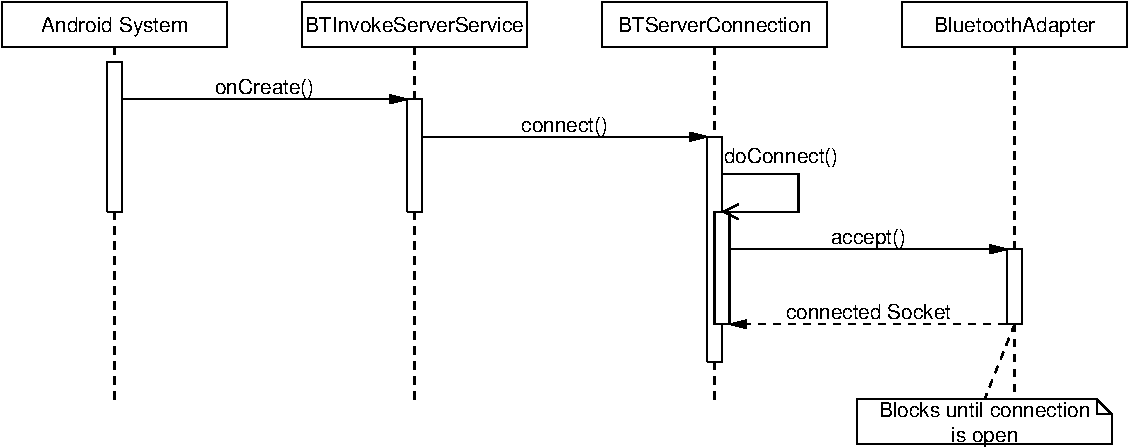
\includegraphics[width=\linewidth,keepaspectratio]{bt_server}
  \caption{Verbindungsaufbau Serverseite}
  \label{fig:bt_server}
\end{figure}
\begin{figure}[htbp]
  \centering
  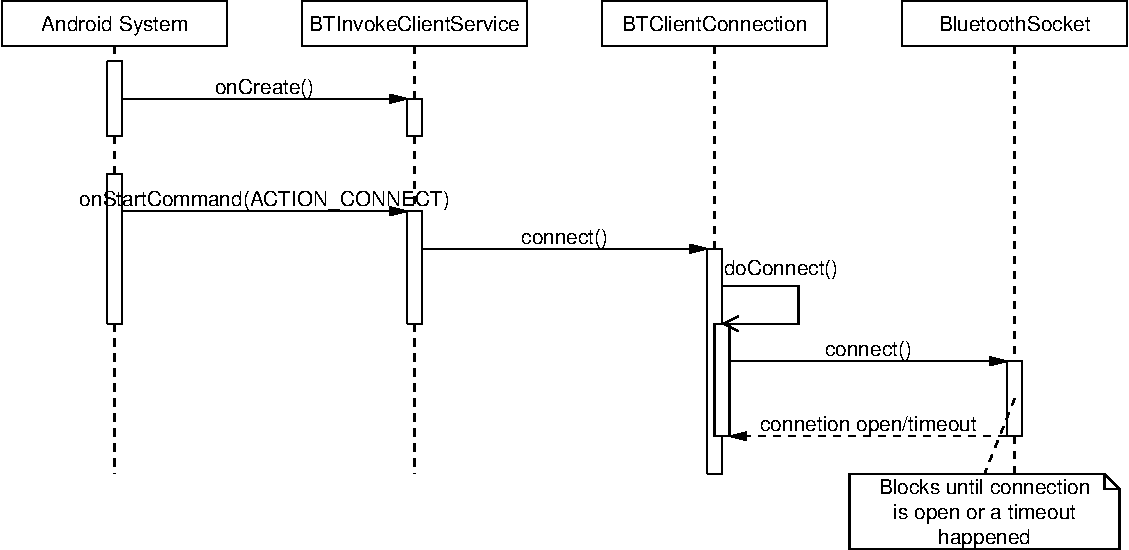
\includegraphics[width=\linewidth,keepaspectratio]{bt_client}
  \caption{Verbindungsaufbau Serverseite}
  \label{fig:bt_client}
\end{figure}
%
\subsection{Aufruf von Methoden über Bluetooth}
%
Um einen String über Bluetooth zu senden braucht das jeweilige Objekt Zugriff auf den \lstinline{InputStream} und \lstinline{OutputStream} der Bluetooth Verbindung. Da das Verbindungsobjekt innerhalb der Services existiert, wurde eine Möglichkeit benötigt den zu sendeten String zum Service zu schicken. Da die Services bereits \emph{Broadcasts} und \emph{BroadcastReciever} verwenden, schien es sinnvoll diese zu verwenden.

Der Aufruf einer Methode über Bluetooth läuft wie folgt ab:
\begin{enumerate}
  \item Benutzer/Activity auf Server- bzw. UI-Seite ruft die statische Methode \lstinline{BTInoke.remoteExecute} auf.
  \item \lstinline{BTInoke.remoteExecute} erstellt ein \lstinline{RemoteInvocationRequest} und sendet ihn als JSON-String über einen Broadcast mit der \emph{Action} \lstinline{BTInvokeMessages.REMOTE_INVOCATION}.
  \item \lstinline{BTInvokeServerService} bekommt den Broadcast, sendet den JSON-String über Bluetooth und wartet auf eine Antwort.
  \item Auf dem Clientgerät empfängt \lstinline{BTInvokeClientService} den JSON-String, konvertiert ihn zurück zu einem \lstinline{RemoteInvocationRequest}-Objekt und ruft die Methode mit dem darin enthaltenen Namen und Parametern auf.
  \item Nachdem die Methode fertig ist erstellt \lstinline{BTInvokeClientService} aus dem Ergebnis ein \lstinline{RemoteInvocationResult}-Objekt und sendet es als JSON-String zurück zum Servergerät.
  \item \lstinline{BTInvokeServerService} empfängt den String und sendet ihn in einem Broadcast mit der \emph{Action} \lstinline{BTInvokeMessages.REMOTE_INVOCATION_RESULT}.
  \item Die Activity die den Aufruf gestartet hat kann nun diesen Broadcast empfangen und daraus das Ergebnis des Methodenaufrufs holen.
\end{enumerate}
\autoref{fig:seq} zeigt den Ablauf nochmal als vereinfachtes Sequenzdiagramm. Weitere Informationen zu den beteiligten Klassen befinden sich im Javadoc.

\begin{sloppypar}
Bevor eine Methode auf der Clientseite ausgeführt werden kann muss sie mit der Methode \lstinline{registerInterfaceAndImplementation} der Klasse \lstinline{BTInvokeMethodManager} registriert werden. Hier gibt es allerdings einige Einschränkungen:
\end{sloppypar}
\begin{itemize}
  \item Es können nicht zwei Interfaces registriert werden die eine Methode mit gleichem Namen besitzen. In so einem Fall würde versucht werden die erste gefundene auszuführen.
  \item Eine Methode in einem Interface darf nicht überladen sein.
  \item Die Methoden können nur primitive Datentypen und String als Parameter oder Rückgabetyp besitzen.
\end{itemize}
In der aktuellen Version bekommt die Activity den JSON-String mit dem Broadcast geschickt und muss das Ergebnis selbst herausholen. Dies ist unschön, allerdings konnte eine bessere Lösung aus Zeitgründen nicht mehr Implementiert werden. 
\begin{figure}[htbp]
  \centering
  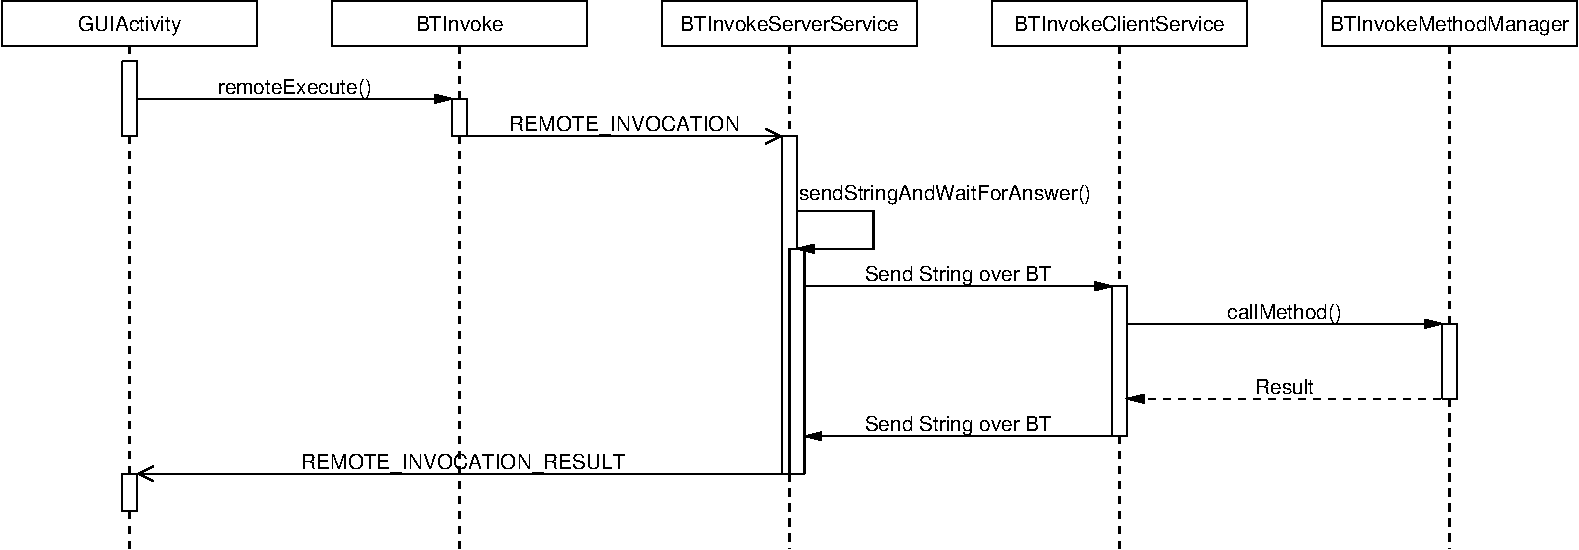
\includegraphics[width=\textwidth,keepaspectratio]{seq}
  \caption{Aufruf einer Methode über Bluetooth}
  \label{fig:seq}
\end{figure}

Es wurde zusätzlich noch eine zweite Variante implementiert, die auf dem vorigen beschriebenen Ablauf aufbaut. Die Klasse \lstinline{Proxy} aus der Java Standard Bibliothek erlaubt es zur Laufzeit ein Interface zu implementieren. Alle aufrufe über das so erstellte Objekte werden von einem Objekt ausgeführt, das das Interface \lstinline{InvocationHandler} implementiert \cite{dpunkt2002}. Somit wirkt der Aufruf für einen Benutzer wie ein lokaler Aufruf. Für diesen Zweck wurde die Klasse \lstinline{BTInvocationHandler} erstellt. Sie lässt sich wie in \autoref{fig:proxy} dargestellt benutzen:
\begin{figure}[hbtp]
  \begin{lstlisting}[basicstyle=\ttfamily\scriptsize]
  // Implemetiere Interface zur Laufzeit
  IExampleInterace e = Proxy.newProxyInstance(getClass().getClassLoader(), new Class<?>[]{IExampleInterace.class}, new BTInvocationHandler(context);
  // Jetzt ist es moeglich eine Methode des Interfaces aufzurufen als waere sie lokal.
  int result = e.exampleMethod(42);
  \end{lstlisting}
  \caption{Beispiel der Proxy-Variante}
  \label{fig:proxy}
\end{figure}
\begin{sloppypar}
\textbf{Wichtige Anmerkung}: Innerhalb von \lstinline{BTInvocationHandler} wird einfach der zuvor genannte Ablauf mit \lstinline{BTInoke.remoteExecute} gestartet. Damit allerdings auch das Ergebnis zurückgegeben werden kann, muss der Aufruf so lange blockieren bis das der Broadcast \lstinline{BTInvokeMessages.REMOTE_INVOCATION_RESULT} angekommen ist. Ein BroadcastReciever wird immer im UI-Thread aufgerufen. Wird nun eine Methode des Interfaces auch auf dem UI-Thread aufgerufen, ist dieser blockiert und der BroadcastReciever kann niemals ausgeführt werden. Somit ist die ganze Applikation blockiert.
\end{sloppypar}
% TODO: Status narichten
\subsection{Tutorial: Benutzung von BTInvoke}
%
Ein Benutzer muss die folgenden Schritte ausführen um BTInvoke zu benutzen:
\begin{sloppypar}
\begin{enumerate}
  \item Clientseite: Registrieren eines Interface mit einer implementierenden Klasse in \lstinline{BTInvokeMethodManager}.
  \item Clientseite: Starten des \lstinline{BTInvokeClientService}.
  \item Serverseite: Starten des \lstinline{BTInvokeServerService}.
  \item Clientseite: Starten des Verbindungsaufbaus mit \lstinline{startService} und dem \lstinline{ACTION_CONNECT} Intent.
  \item Serverseite, falls Proxyvariante: Erstellung einer Proxyimplementierung mit \lstinline{Proxy.newProxyInstance} und \lstinline{BTInvocationHandler}.
  \item Serverseite: Starten des Methodenaufrufs durch Broadcast oder Proxyvariante.
  \item Serverseite: Warten auf Antwort und Ergebnis verwenden.
\end{enumerate}
\end{sloppypar}
%
\phantomsection
\begin{sidewaysfigure}
  %\centering
  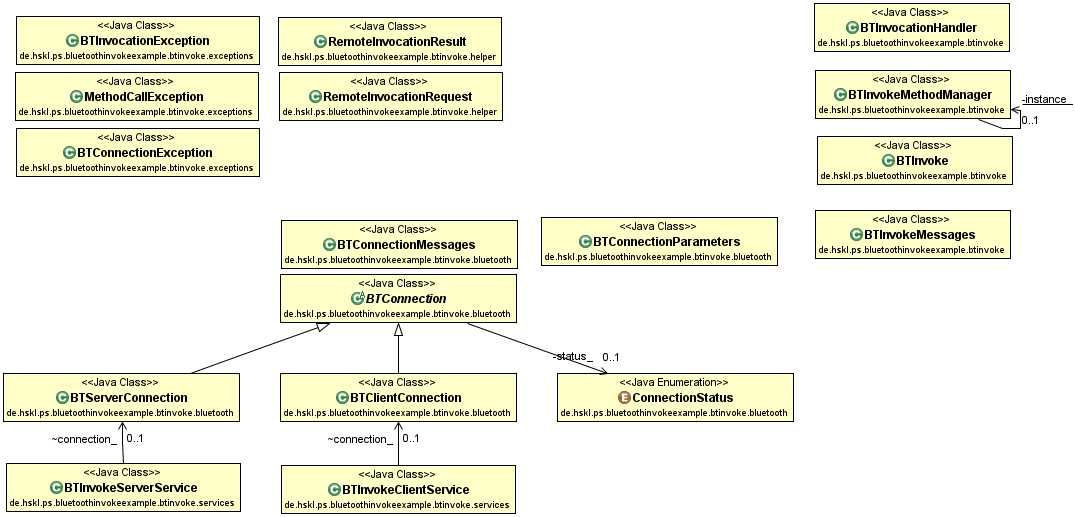
\includegraphics[width=\textheight,keepaspectratio]{classes}
  \caption{Übersicht über alle erstellen Klassen. Erstellt mit Objectaid für Eclipse(\url{objectaid.com}) }
\end{sidewaysfigure}
%